\section{Versuchsdurchführung}
\label{sec:durchfuehrung}
\subsection{Versuchsaufbau}
\label{sec:aufbau}

Für den Versuch wurde eine Anordnung entsprechend der Darstellung verwendet. Das Zählrohr wird hinter einer 
Blei-Abschirmung platziert um den Einfluss des Nulleffektes zu minimieren. Die vom Zählrohr registrierten 
Impulse werden an einen Zähler weitergeleitet, an welchem das gewünschte Messintervall $\Delta t$ eingestellt 
werden kann. Er besitzt zwei Anzeigevorrichtungen, zwischen denen nach $\Delta t$ umgeschaltet wird, sodass 
zu jedem Zeitpunkt eine der Anzeigen zählt und die jeweils andere das Ergebnis des vorrangegangenen 
Zeitintervalls anzeigt.
\begin{figure}
    \centering
    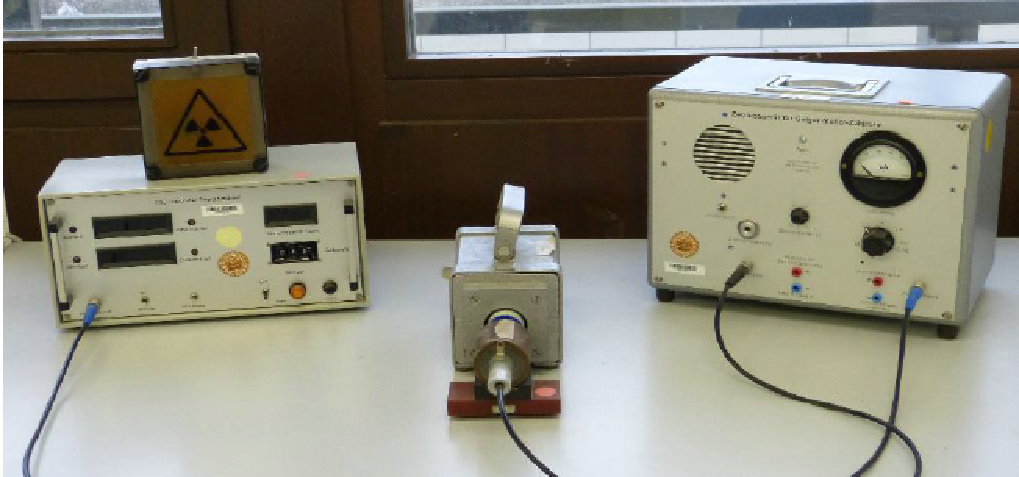
\includegraphics{aufbau.pdf}
    \caption{Versuchsaufbau, Quelle:1.}
    
  \end{figure}

\subsection{Messungen}
\label{sec:messungen}
Zunächst wurde der Nulleffekt gemessen, wobei ein großes Zeitintervall von $\Delta t=300$ s verwendet 
wurde, um den Messfehler zu minimieren. \\
Anschließend wurden Messwerte für das Vanadium direkt nach Aktivierung der Probe erhoben, dabei wurde 
als Zeitintervall $\Delta t=30$ s gewählt. Eine analoge Messung wurde für Rhodium durchgeführt, jedoch 
mit einer Messzeit von $\Delta t=15$ s.  